%%%%%%%%%%%%%%%%%%%%%%%%%%%%%%%%%%%%%%%%%
% Masters/Doctoral Thesis 
% LaTeX Template
% Version 2.5 (27/8/17)
%
% This template was downloaded from:
% http://www.LaTeXTemplates.com
%
% Version 2.x major modifications by:
% Vel (vel@latextemplates.com)
%
% This template is based on a template by:
% Steve Gunn (http://users.ecs.soton.ac.uk/srg/softwaretools/document/templates/)
% Sunil Patel (http://www.sunilpatel.co.uk/thesis-template/)
%
% Template license:
% CC BY-NC-SA 3.0 (http://creativecommons.org/licenses/by-nc-sa/3.0/)
%
%%%%%%%%%%%%%%%%%%%%%%%%%%%%%%%%%%%%%%%%%

%----------------------------------------------------------------------------------------
%	PACKAGES AND OTHER DOCUMENT CONFIGURATIONS
%----------------------------------------------------------------------------------------
\PassOptionsToPackage{spanish,english}{babel}
\documentclass[
11pt, % The default document font size, options: 10pt, 11pt, 12pt
%oneside, % Two side (alternating margins) for binding by default, uncomment to switch to one side
english, % ngerman for German
singlespacing, % Single line spacing, alternatives: onehalfspacing or doublespacing
%draft, % Uncomment to enable draft mode (no pictures, no links, overfull hboxes indicated)
%nolistspacing, % If the document is onehalfspacing or doublespacing, uncomment this to set spacing in lists to single
%liststotoc, % Uncomment to add the list of figures/tables/etc to the table of contents
%toctotoc, % Uncomment to add the main table of contents to the table of contents
%parskip, % Uncomment to add space between paragraphs
%nohyperref, % Uncomment to not load the hyperref package
headsepline, % Uncomment to get a line under the header
%chapterinoneline, % Uncomment to place the chapter title next to the number on one line
%consistentlayout, % Uncomment to change the layout of the declaration, abstract and acknowledgements pages to match the default layout
]{MastersDoctoralThesis} % The class file specifying the document structure

\usepackage[utf8]{inputenc} % Required for inputting international characters
\usepackage[T1]{fontenc} % Output font encoding for international characters

\usepackage{mathpazo} % Use the Palatino font by default

%\usepackage[backend=bibtex,style=authoryear,natbib=true]{biblatex} % Use the bibtex backend with the authoryear citation style (which resembles APA)

\usepackage[backend=bibtex,style=numeric,natbib=true,sorting=none]{biblatex} % Use the bibtex backend with the authoryear citation style (which resembles APA)
%\usepackage{cite}
\addbibresource{example.bib} % The filename of the bibliography
%\bibliography{example.bib}
\usepackage[autostyle=true]{csquotes} % Required to generate language-dependent quotes in the bibliography

%----------------------------------------------------------------------------------------
%	MARGIN SETTINGS
%----------------------------------------------------------------------------------------

\geometry{
	paper=a4paper, % Change to letterpaper for US letter
	inner=2.5cm, % Inner margin
	outer=3.8cm, % Outer margin
	bindingoffset=.5cm, % Binding offset
	top=1.5cm, % Top margin
	bottom=1.5cm, % Bottom margin
	%showframe, % Uncomment to show how the type block is set on the page
}

%----------------------------------------------------------------------------------------
%	THESIS INFORMATION
%----------------------------------------------------------------------------------------

\thesistitle{Integración de LibreMesh para Incentived Mesh Networking} % Your thesis title, this is used in the title and abstract, print it elsewhere with \ttitle
\supervisor{Dr. Claudio \textsc{Delrieux} \\ Dr. Eduardo \textsc{Paolini} \\ Dr. Carlos \textsc{Matrángolo}} % Your supervisor's name, this is used in the title page, print it elsewhere with \supname
\examiner{} % Your examiner's name, this is not currently used anywhere in the template, print it elsewhere with \examname
\degree{Ingeniero Electrónico} % Your degree name, this is used in the title page and abstract, print it elsewhere with \degreename
\author{Luciano \textsc{Bruna}} % Your name, this is used in the title page and abstract, print it elsewhere with \authorname
\addresses{} % Your address, this is not currently used anywhere in the template, print it elsewhere with \addressname

\subject{Mesh Networking} % Your subject area, this is not currently used anywhere in the template, print it elsewhere with \subjectname
\keywords{} % Keywords for your thesis, this is not currently used anywhere in the template, print it elsewhere with \keywordnames
\university{\href{http://www.uns.edu.ar}{Universidad Nacional del Sur}} % Your university's name and URL, this is used in the title page and abstract, print it elsewhere with \univname
\department{\href{http://www.diec.uns.edu.ar/}{Departamento de Ingeniería Eléctrica y Computadoras}} % Your department's name and URL, this is used in the title page and abstract, print it elsewhere with \deptname
\group{\href{http://researchgroup.university.com}{Research Group Name}} % Your research group's name and URL, this is used in the title page, print it elsewhere with \groupname
\faculty{\href{http://uns.edu.ar}{Universidad Nacional del Sur}} % Your faculty's name and URL, this is used in the title page and abstract, print it elsewhere with \facname

\AtBeginDocument{
\hypersetup{pdftitle=\ttitle} % Set the PDF's title to your title
\hypersetup{pdfauthor=\authorname} % Set the PDF's author to your name
\hypersetup{pdfkeywords=\keywordnames} % Set the PDF's keywords to your keywords
}

\newcaptionname{spanish}{\acknowledgementname}{Agradecimientos}
\newcaptionname{spanish}{\byname}{por}
\newcaptionname{spanish}{\abbreviationsname}{Lista de Abreviaciones}
%\newcaptionname{spanish}{\Authorshipname}{Autoría}
%\providecaptionname{spanish}{\declaration}{Declaración de Autoría}




\begin{document}

\frontmatter % Use roman page numbering style (i, ii, iii, iv...) for the pre-content pages

\pagestyle{plain} % Default to the plain heading style until the thesis style is called for the body content

%----------------------------------------------------------------------------------------
%	TITLE PAGE
%----------------------------------------------------------------------------------------

\begin{titlepage}
\begin{center}

\vspace*{.06\textheight}
{\scshape\LARGE \univname\par}\vspace{1.5cm} % University name
\textsc{\Large Tesis de Grado}\\[0.5cm] % Thesis type

\HRule \\[0.4cm] % Horizontal line
{\huge \bfseries \ttitle\par}\vspace{0.4cm} % Thesis title
\HRule \\[1.5cm] % Horizontal line
 
\begin{minipage}[t]{0.4\textwidth}
\begin{flushleft} \large
\emph{Autor:}\\
\href{http://www.linkedin.com/in/lucianobruna}{\authorname} % Author name - remove the \href bracket to remove the link
\end{flushleft}
\end{minipage}
\begin{minipage}[t]{0.4\textwidth}
\begin{flushright} \large
\emph{Directores:} \\
%\href{http://www.jamessmith.com}{\supname} % Supervisor name - remove the \href bracket to remove the link  
\href{https://www.linkedin.com/in/claudio-delrieux-3308091}{Dr. Claudio \textsc{Delrieux}}\\
\href{https://www.linkedin.com/in/eduardo-paolini-9768536}{Dr. Eduardo \textsc{Paolini}}\\
\href{https://www.linkedin.com/in/carlos-matrangolo-16991a51/}{Dr. Carlos \textsc{Matrángolo}}
\end{flushright}
\end{minipage}\\[3cm]
 
\vfill

%\large \textit{Una tesis presentada para el cumplimiento de los requisitos\\ para el título de \degreename}\\[0.3cm] % University requirement text
%\textit{en el}\\[0.4cm]
%\groupname\\
\deptname\\[8cm] % Research group name and department name
 
\vfill

{\large \today}\\[10cm] % Date
%\includegraphics{Logo} % University/department logo - uncomment to place it
 
\vfill
\end{center}
\end{titlepage}

%----------------------------------------------------------------------------------------
%	DECLARATION PAGE
%----------------------------------------------------------------------------------------

%\begin{declaration}
%\addchaptertocentry{\authorshipname} % Add the declaration to the table of contents
%\noindent Yo, \authorname, declaro que esta tesis llamada, \enquote{\ttitle} y el trabajo %presentado son míos. Confirmo que:

%\begin{itemize} 
%\item Este trabajo fue realizado completa o parcialmente while in candidature for a research degree at this University.
%\item Where any part of this thesis has previously been submitted for a degree or any other qualification at this University or any other institution, this has been clearly stated.
%\item Where I have consulted the published work of others, this is always clearly attributed.
%\item Cada vez que he consultado trabajos publicados por otros, se ha hecho la atribución correspondiente.
%\item Where I have quoted from the work of others, the source is always given. With the exception of such quotations, this thesis is entirely my own work.
%\item Cada vez que he citado el trabajo de otros, la fuente siempre ha sido dada. Con la excepción de tales citaciones, esta tesis es enteramente mía.
%\item I have acknowledged all main sources of help.
%\item He reconocido todas las fuentes de ayuda a mi trabajo.
%\item Where the thesis is based on work done by myself jointly with others, I have made clear exactly what was done by others and what I have contributed myself.\\
%\end{itemize}
 
%\noindent Firma:\\
%\rule[0.5em]{25em}{0.5pt} % This prints a line for the signature
 
%\noindent Fecha:\\
%\rule[0.5em]{25em}{0.5pt} % This prints a line to write the date
%\end{declaration}


%\cleardoublepage

%----------------------------------------------------------------------------------------
%	QUOTATION PAGE
%----------------------------------------------------------------------------------------

\vspace*{0.2\textheight}

%\noindent\enquote{\itshape Thanks to my solid academic training, today I can write hundreds of words on virtually any topic without possessing a shred of information, which is how I got a good job in journalism.}\bigbreak

\noindent\enquote{\itshape Cuando cambiamos la forma de ver las cosas, las cosas cambian (aca iria una frase como la gente, afín al trabajo y con la que me identifique, si es que llegase a encontrar una, sino esta pagina se omite).}\bigbreak

\hfill Wayne Dyer

%----------------------------------------------------------------------------------------
%	ABSTRACT PAGE
%----------------------------------------------------------------------------------------

\begin{abstract}
\addchaptertocentry{\abstractname} % Add the abstract to the table of contents
%The Thesis Abstract is written here (and usually kept to just this page). The page is kept centered vertically so can expand into the blank space above the title too\ldots

Acá iría el abstracto, un resumen de todo lo que hice. Podria tener un poquito de narrativa tensional tal y como menciono claudio. "se vio ante tal o cual eventualidad, las redes mesh son la posible solucion. Investigando redes mesh e incursionando en el termino incentived mesh, se detecto que althea y libremesh podrian integrarse y mejorar asi el avance de ambos grupos." Pero no mucho, la idea es que aca en el abstracto va todo mas resumido y serio. En cambio, mas adelante en la introduccion iria mas narrativa que atrape al lector no experto en el tema.


%aca iría algo de narrativa tensional similar a lo que sugirió claudio. "se vio ante tal o cual eventualidad, las redes mesh son la posible solucion. Investigando redes mesh e incursionando en el termino incentived mesh, se detecto que althea y libremesh podrian integrarse y mejorar asi el avance de ambos grupos." Algo así

\end{abstract}

%----------------------------------------------------------------------------------------
%	ACKNOWLEDGEMENTS
%----------------------------------------------------------------------------------------

\begin{acknowledgements}
\addchaptertocentry{\acknowledgementname} % Add the acknowledgements to the table of contents
%The acknowledgments and the people to thank go here, don't forget to include your project adviso\ldots
Esto para mi es muy importante, no solo agradecer a mis directores y advisors sino tambien a Nicolas Pace, Althea. Aca irian los agradecimientos
\end{acknowledgements}

%----------------------------------------------------------------------------------------
%	LIST OF CONTENTS/FIGURES/TABLES PAGES
%----------------------------------------------------------------------------------------

\tableofcontents % Prints the main table of contents

\listoffigures % Prints the list of figures

\listoftables % Prints the list of tables

%----------------------------------------------------------------------------------------
%	ABBREVIATIONS
%----------------------------------------------------------------------------------------

\begin{abbreviations}{ll} % Include a list of abbreviations (a table of two columns)

\textbf{SSID} & \textbf{S}ervice \textbf{S}et \textbf{I}dentifier\\
\textbf{BATMAN} & \textbf{B}etter \textbf{A}pproach \textbf{T}o \textbf{M}obile \textbf{A}d-hoc \textbf{N}etworks\\
\textbf{WCN} & \textbf{W}ireless \textbf{C}ommunity \textbf{N}etworks\\
\textbf{MANET} & \textbf{M}obile \textbf{A}d-Hoc \textbf{NET}works\\
\textbf{MPR} & \textbf{M}ulti \textbf{P}oint \textbf{R}elay\\
\textbf{OLSR} & \textbf{O}ptimized \textbf{L}ink \textbf{S}tate \textbf{R}outing \\

\end{abbreviations}

%----------------------------------------------------------------------------------------
%	PHYSICAL CONSTANTS/OTHER DEFINITIONS
%----------------------------------------------------------------------------------------

%\begin{constants}{lr@{${}={}$}l} % The list of physical constants is a three column table

% The \SI{}{} command is provided by the siunitx package, see its documentation for instructions on how to use it

%Speed of Light & $c_{0}$ & \SI{2.99792458e8}{\meter\per\second} (exact)\\
%Constant Name & $Symbol$ & $Constant Value$ with units\\

%\end{constants}

%----------------------------------------------------------------------------------------
%	SYMBOLS
%----------------------------------------------------------------------------------------

%\begin{symbols}{lll} % Include a list of Symbols (a three column table)

%$a$ & distance & \si{\meter} \\
%$P$ & power & \si{\watt} (\si{\joule\per\second}) \\
%Symbol & Name & Unit \\

%\addlinespace % Gap to separate the Roman symbols from the Greek

%$\omega$ & angular frequency & \si{\radian} \\

%\end{symbols}

%----------------------------------------------------------------------------------------
%	DEDICATION
%----------------------------------------------------------------------------------------

\dedicatory{Dedicado a Diana Sanchez\ldots} 

%----------------------------------------------------------------------------------------
%	THESIS CONTENT - CHAPTERS
%----------------------------------------------------------------------------------------

\mainmatter % Begin numeric (1,2,3...) page numbering

\pagestyle{thesis} % Return the page headers back to the "thesis" style

% Include the chapters of the thesis as separate files from the Chapters folder
% Uncomment the lines as you write the chapters

% Chapter 1

\chapter{Introduccion} % Main chapter title

\label{Chapter1} % For referencing the chapter elsewhere, use \ref{Chapter1} 

%----------------------------------------------------------------------------------------

% Define some commands to keep the formatting separated from the content 
\newcommand{\keyword}[1]{\textbf{#1}}
\newcommand{\tabhead}[1]{\textbf{#1}}
\newcommand{\code}[1]{\texttt{#1}}
\newcommand{\file}[1]{\texttt{\bfseries#1}}
\newcommand{\option}[1]{\texttt{\itshape#1}}

%----------------------------------------------------------------------------------------

Durante los últimos años, las redes mesh \footnote{Una red mesh es una topología de red local en la que la infraestructura de nodos (routers, Access Points y otros dispositivos) se conectan directamente, dinámicamente y sin jerarquía a tantos otros nodos como sea posible cooperando entre todos para hacer ruteo de la forma más eficiente posible.} han pasado de ser un concepto teórico de red a convertirse en dispositivos comercialmente disponibles que prometen crear redes distribuídas, capaces de crear links entre sí y mantenerlos autónomamente. El IEEE creó el grupo de trabajo 802.11s, que define cómo los dispositivos inalámbricos pueden interconectarse para crear una red  mesh inalámbrica \cite{IEEE802WIKIPEDIA}. Esto tiene la intención de guiar a institutos de investigación y a la industria para desarrollar un estándar para redes mesh, con el objetivo de proveer interoperabilidad entre todos los dispositivos. Mientras el estándar 802.11 sigue bajo desarrollo, hay un número de protocolos de red que están actualmente disponibles.

De todas las aplicaciones de redes mesh, en este trabajo se destacan las redes mesh comunitarias no cableadas, o mesh WCNs (Mesh Wireless Comunity Networks), cuya topología está representada en la figura (\ref{MWCNfigura1}). Estas han sido desarrolladas como movimientos de entusiastas de redes no cabledas, quienes usando equipamiento de bajo costo para una interconexión gratuita, han creado redes completamente autónomas. Su aparición se debe principalmente a la búsqueda de estos grupos de lograr un servicio equivalente a los ofrecidos por redes 2.5G y 3G pero de manera gratuita\cite{PAPERcitadoPORalthea}. 

\begin{figure}[th]	
	\centering	
	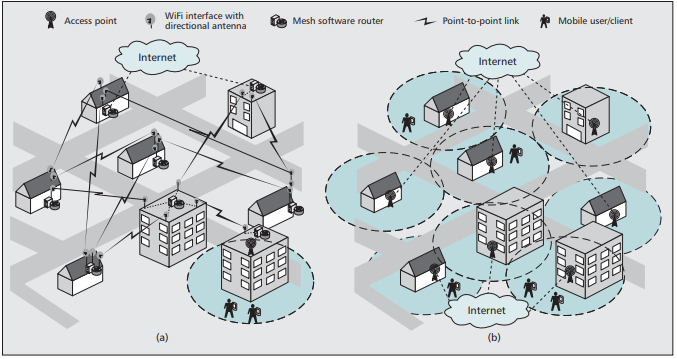
\includegraphics[width=0.95\textwidth]{./figures/WCNs1}		
	\caption{\textit{Topología de redes mesh WCNs. (falta cortar la foto por la mitad y traducirla al castellano)}}
	\label{MWCNfigura1}
\end{figure}



Las razones para participar en una red mesh son muy variadas. Aquellas personas que creen que la conectividad de banda ancha debería ser libre y gratuita y que las barreras impuestas por los oligopolios de los ISPs deben ser eliminadas usualmente son los primeros en unirse a WCNs. En el cuadro (\ref{cuadroWCNS1}), se reportan algunas de las mesh WCNs más significativas a nivel mundial categorizadas según el año en que han sido diseñadas y la cantidad de nodos. Cabe destacar que todas ellas parten de una iniciativa comunitaria, es decir que son el resultado de efuerzos colectivos de voluntarios individuales y funcionan sin fines de lucro.

\begin{table}[th]
\centering
\caption{Comunidades de redes mesh WCNs en todo el mundo.}
\label{cuadroWCNS1}
\begin{tabular}{|c|c|c|c|}
\hline
\textbf{\begin{tabular}[c]{@{}c@{}}Nombre\\   de la Red\end{tabular}} & \textbf{Ubicación}                                                       & \textbf{\begin{tabular}[c]{@{}c@{}}Año de\\   Fundación\end{tabular}} & \textbf{\begin{tabular}[c]{@{}c@{}}Cantidad de\\   nodos\end{tabular}} \\ \hline
SeattleWireless                                                       & \begin{tabular}[c]{@{}c@{}}Seattle, WA, Estados\\   Unidos\end{tabular}  & 2000                                                                  & 80                                                                     \\ \hline
AWMN                                                                  & Athena, Grecia                                                           & 2002                                                                  & 2473                                                                   \\ \hline
CUWiN                                                                 & \begin{tabular}[c]{@{}c@{}}Urbana, IL, Estados\\   Unidos\end{tabular}   & 2002                                                                  & 48                                                                     \\ \hline
\begin{tabular}[c]{@{}c@{}}Berlin's\\   Freifunk\end{tabular}         & Berlin, Alemania                                                         & 2002                                                                  & 316                                                                    \\ \hline
\begin{tabular}[c]{@{}c@{}}Wireless\\   Leiden\end{tabular}           & Leiden, Países Bajos                                                     & 2002                                                                  & 73                                                                     \\ \hline
\begin{tabular}[c]{@{}c@{}}NetEquality\\   Roofnet\end{tabular}       & \begin{tabular}[c]{@{}c@{}}Portland, OR, Estados\\   Unidos\end{tabular} & 2007                                                                  & 126                                                                    \\ \hline
NYCwireless                                                           & \begin{tabular}[c]{@{}c@{}}New York, Estados\\   Unidos\end{tabular}     & 2001                                                                  & 145                                                                    \\ \hline
\end{tabular}
\end{table}

En el estudio de este fenómeno, se destacó la iniciativa de la empresa Althea, con la cual se desarrolló este trabajo en conjunto. Althea propone un modelo de negocios basado en el incentivized mesh \footnote{Explicar con palabras mas bonitas que el incentivized mesh es basicamente pagarle a la gente para que comparta un poquito de su ancho de banda.}. Y aca explicar un poquito brevemente qué hace althea (basicamente copipastear la primera parte de su white paper sin entrar en detalles tecnicos de que tipos de nodos tienen, etc.).

En este parrafo explicar un poco la problematica y el hecho de que me di cuenta (hablar siempre en voz pasiva xq sino me agarra toc) que podría integrar las plataformas althea con libremesh (y explicar qué es libremesh usando el pie de página, no hace falta mas en esta instancia ya que lo explicare por completo en la seccion del marco teorico).

En este parrafo explicar brevemente (pero no tan breve como en el resumen) todo lo que hice en el trabajo y las cosas que quedan como propuesta para seguir trabajando en el futuro.

Y en este parrafo poner -en la seccion 1- se vera tal cosa. En el -capitulo 2- tal otra cosa y listo. Es una manera util de ocupar espacio (mas de la mitad de los papers que lei lo hacen asi que yo tambien lo hare). 

% Chapter Template

\chapter{Marco Teórico} % Main chapter title

\label{Chapter2} % Change X to a consecutive number; for referencing this chapter elsewhere, use \ref{ChapterX}

%----------------------------------------------------------------------------------------
%	SECTION 1
%----------------------------------------------------------------------------------------

Este capítulo está pensado para dar el $background$ necesario para entender a las redes mesh y algunos algoritmos de ruteo específicos. Estos han sido partícipes de discusiones por parte de las entidades protagonistas de este proyecto. Además se incursiona en temas como criptografía y ..


Mencionar aca o en algun lado que esto es muy importante para entender por que libremesh usa los protocolos que usa y por que althea usa lo que usa, etc.

\section{Definiciones Iniciales}

\subsection{Redes Ad Hoc y Redes Mesh}

En gran parte de la bibliografía consultada, se han utilizado los términos redes ad hoc y redes mesh de manera indistinta. Si bien esto no representa ningún error en esos casos, puede generar confusiones si no se conoce la diferencia entre ellos. Por eso es importante destacarla.

Una red Ad hoc implica el compromiso cooperativo de un conjunto de nodos wireless sin ningún tipo de intervención por parte de algún access point centralizado o de alguna infraestructura existente. Este tipo de red tiene características claves de ser auto-generativas y auto-curativas y no depender de ningún servicio centralizado de ningún nodo en particular. Una red Ad-hoc puede ser wireless, en cuyo caso sus dispositivos, tales como laptops o sensores, realizan una función de ruteo para enviarse datos creando una forma arbitraria de topología de red. Cuando todos los dispositivos son móviles, se habla de redes MANET \footnote{MANET: Abreviación de Mobile Ad-Hoc Network.}, que pueden cambiar de topología muy rápidamente y de forma impredecible. Redes de sensores no cableados son un buen ejemplo de redes MANET.

Una red wireless mesh se caracteriza por tener routers estáticos o cuasi-estáticos dedicados que tienen el trabajo de realizar la función de ruteo de paquetes a lo largo de la red. Además, están los dispositivos clientes, quienes no tienen funcionalidad de ruteo. Estos están conectados a los ruters wireless. 

Existen muchos protocolos de ruteo compatibles con estos tipos de redes. La gran mayoría de ellos parte de grupos académicos que buscan optimizar diferentes cuestiones como la velocidad de convergencia o la evitación de lazos de ruteo. A estos se les prestará una mayor atención en la sección (\ref{SeccionProtocolosDeRuteo}). Además, el grupo de trabajo 802.11s de la IEEE define un estándar para las redes mesh en donde se define, entre otras cosas, el método de ruteo para este tipo de redes.

\section{Protocolos de Ruteo}
\label{SeccionProtocolosDeRuteo}

Los protocolos para redes mesh se clasifican en tres categorías: $reactivos$, $proactivos$ e $hibridos$ \cite{PAPERrealWORLDperformance}. Los protocolos reactivos solo buscan un camino entre nodos cuando hay datos para ser enviados. Este método tiene la ventaja de no gastar ancho de banda de la red con mensajes de control cuando la transmisión de datos no es requerida. Los protocolos reactivos idealmente se utilizan en redes Ad Hoc donde con los nodos móviles los caminos de datos podrían cambiar contínuamente.

Por otro lado, los protocolos proactivos actívamente establecen y mantienen caminos de datos para nodos tanto si los datos necesitan ser enviados o no. Esto permite una latencia menor a la hora de enviar datos a través de la red ya que el camino óptimo ya es conocido. De todas maneras, esto viene con un costo computacional mayor y con la necesidad de una administración de red mucho más compleja.

Los protocolos híbridos exhiben las propiedades de tanto los protocolos proactivos y reactivos. En general, intentan usar características proactivas o reactivas según el escenario, lo cual explota sus fortalezas y es por eso que pueden lograr un mayor nivel de escalabilidad. En general, son más complejos en comportamiento, lo cual hace que sean más complejos de implementar que los protocolos puramente proactivos o reactivos.

En (\ref{subseccionAlgoritmoVectorDistancia}) se explicará el algoritmo $Vector$ $Distancia$ que es la base de varios protocolos de ruteo muy conocidos como RIP y OLSR. Se pondrá en discusión la característica principal y la problemática de este último en (\ref{subseccionProtocoloOLSR}). Luego se detallarán protocolos más eficientes para redes mesh en las secciones (\ref{subseccionProtocoloBatman}), (\ref{subseccionProtocoloBabel}) y (\ref{subseccionProtocoloSSR}). Finalmente, en (\ref{subseccionComparacionesProtocolosDeRuteo}) se compararán todos los protocolos previamente descritos.

\subsection{Algoritmo Vector-Distancia}
\label{subseccionAlgoritmoVectorDistancia}

El algoritmo $Vector$ $Distancia$ se trata de uno de los más importantes junto con el $estado$ $de$ $enlace$ \footnote{El estado de enlace es .....}. Se basa en el algoritmo de Bellman-Ford para calcular las rutas. Requiere que un router informe a sus vecinos de los cambios en la topología periódicamente y en algunos casos cuando se detecta un cambio en la topología de la red.

Se basa en calcular la dirección y la distancia hasta cualquier enlace en la red. El costo de alcanzar un destino se lleva a cabo usando cálculos matemáticos como la métrica del camino. Una de las métricas más utilizadas es el número de $hops$ \footnote{En una red, se le dice $hop$ a una porción de camino entre una fuente y su destino. La cuenta de $hops$ se refiere al número de dispositivos intermediarios a través de los cuales deben pasar los datos.}.

Los cambios son detectados periódicamente ya que la tabla de enrutamiento de cada router se envía a todos los vecinos que usan el mismo protocolo. Una vez que el router tiene toda la información, actualiza su tabla e informa a sus vecinos de los mismos. Este proceso se conoce también como $enrutamiento$ $por$ $rumor$ ya que los nodos utilizan la información de sus vecinos y no pueden comprobar a ciencia cierta si ésta es verdadera o no.

El algoritmo de Bellman-Ford se adapta perfectamente al modo de aprendizaje de los nodos que “nacen”, es decir, cuando se conectan a la red. A medida que el algoritmo progresa, el nuevo nodo va adquiriendo más información sobre el resto de nodos de la red. Este algoritmo converge rápidamente cuando se conectan nuevos nodos. Por ello se suele decir que las buenas noticias viajan rápido por la red.

Un problema del que padece este algoritmo es el de la transmisión de malas noticias por la red tales como la ruptura de un enlace o la desaparición de un nodo. Este algoritmo converge lentamente en estos casos. Aunque el principal inconveniente de este algoritmo es el de la cuenta a infinito. Para ilustrarlo, se puede tomar como ejemplo el de la figura (\ref{figuraVectorDistancia1}).

\begin{figure}[th]	
	\centering	
	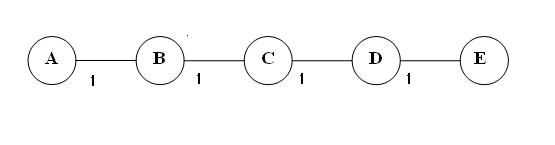
\includegraphics[width=0.95\textwidth]{./figures/VectorDistancia1}		
	\caption{\textit{Topología de red para ejemplificar la limitación del protocolo $vector$ $distancia$.}}
	\label{figuraVectorDistancia1}
\end{figure}

\begin{itemize}
\item Inicialmente A está desactivado. Cuando A se activa, B se entera de que A existe al recibir su vector distancia y actualizar su tabla indicando que A dista 1.

\item El nodo C se entera de que A existe porque B le indica que tiene un enlace hacia A de coste 1. Entonces C actualiza su tabla registrando una trayectoria hacia A de coste 2.

\item Si el nodo A se desconecta entonces B no recibe el VD de A. Sin embargo el nodo C le dice que tiene una trayectoria hasta A de distancia 2. B no sabe que la trayectoria de C a A pasa por el mismo y por tanto cree que puede llegar a A a través de C por lo que actualiza su tabla registrando la distancia 2 + 1 = 3 hasta A.

\item En el siguiente intercambio, el nodo C comprueba que sus vecinos B y D tienen una trayectoria hasta A de distancia 3. C calcula su propia distancia hasta A en 3 + 1 = 4. En los siguientes intercambios, los nodos elevan ilimitadamente su distancia a A (cuenta a infinito).
\end{itemize}

Mientras no se interrumpa la cuenta a infinito, el algoritmo no converge. Aunque se han propuesto diversas soluciones a este problema. El protocolo RIP establece el siguiente criterio:

\begin{center}
$ \infty = 16. $
\end{center}

Es decir, cuando la cantidad de incrementos de distancia supera los 15 en un período de tiempo relativamente corto, RIP considera que se está en un loop infinito y corta las iteraciones. El protocolo OLSR utiliza un acercamiento más eficiente, como se verá en (\ref{subseccionProtocoloOLSR}).


\subsection{Protocolo OLSR}
\label{subseccionProtocoloOLSR}

El protocolo de ruteo Optimized Link State Routing (o OLSR) emplea el algoritmo de $vector$ $distancia$ pero tiene muchos menos conteos a ínfinitos que el protocolo RIP. Para mantener informados a los nodos de la red de los cambios topológicos de la misma, utiliza el mecanimo Multi-Point Relay (o MPR) para hacer flooding \footnote{Se le dice $flooding$ a la acción de enviar un paquete de actualización de métricas a $todos$ los nodos de la red. Cuando un nodo desea hacer $flooding$ primero le envía el paquete deseado a todos sus nodos vecinos. Luego, estos retransmiten el mensaje hasta que éste llegue a todos los nodos de la red.}. A diferencia del flooding convencional, el método MPR evita que todos los nodos vecinos retransmitan los paquetes. Todos los nodos de la red seleccionan entre sus vecinos un conjunto de retransmisores  (o $multi$ $point$ $relays$) encargados de retransmitir los mensajes que envía el nodo inicial. Los demas vecinos del nodo no pueden retransmitir, lo cual reduce significativamente el tráfico generado respecto al flooding tradicional.

Hay varios criterios para elegir los MPRs de un nodo. En general, se considera que el conjunto de MPRs de un nodo debe verificar que son capaces de alcanzar a todos los vecinos situados a 2 $hops$ del nodo que los define como MPR.

EL protocolo OLSR es un protocolo muy usado pero como fue desarrollado en los inicios del 2000 no está pensado para rutear información en redes mesh. De hecho, hay multiples fuentes que demuestran que OLSR sufre de muchos conteos a infinito en redes mesh \cite{PAPERbatman} y que su performance con respecto a otros protocolos de ruteo como los que se presentarán en (\ref{subseccionProtocoloBatman}), (\ref{subseccionProtocoloBabel}) y (\ref{subseccionProtocoloSSR}) es mucho menor \cite{PAPERrealWORLDperformance}.

\subsection{Protocolo BatMan}
\label{subseccionProtocoloBatman}

Mencionar la existencia de BMX7 y diferenciarlo de batman base

\subsection{Protocolo Babel}
\label{subseccionProtocoloBabel}

\subsection{Protocolo SSR}
\label{subseccionProtocoloSSR}

\subsection{Comparaciones}
\label{subseccionComparacionesProtocolosDeRuteo}
Aca podria copi-pastear el cuadro que uso el flaco de althea para su presentacion. El problema es que en ese cuadro hay 2 protocolos que no estudie. SSR porque no lo entendi y CJS... porque no estaba en ningun paper recomendado. Hay que achicar la tabla.

Aca tambien nombrar en algun momento que se puede demotrar que hay muchas brechas de seguridad (y nombrar el paper que dijo eso) y que para llegar a tener un protocolo seguro habria que definir y estandarizar un conjunto de criterios de protocolo seguro ( y citar el paper que dijo eso). Pero que no se le va a dar mucha importancia en este trabajo porque para redes que no sean militares o de informacion fiscal no hace falta (citar al paper que dijo eso ultimo tambien) y yo voy a usar redes caseras.

\section{Criptografía}

\subsection{Hashing}



 
% Chapter 1

\chapter{Aplicaciones Reales de Redes Mesh} % Main chapter title

\label{Chapter1} % For referencing the chapter elsewhere, use \ref{Chapter1} 

\section{LibreMesh}

\section{Althea}

\section{Ammbr}

Ammbr es como althea pero pinta mas a largo plazo, por ahi estaria bueno mencionar algo. y luego en el siguiente capitulo mencionar por que se decidio trabajar con althea en vez de ammbr. La razon es que althea esta mas avanzado y sería mas "directa" la integracion.
% Chapter Template
\chapter{Trabajo Realizado} % Main chapter title

\label{Chapter2} % Change X to a consecutive number; for referencing this chapter elsewhere, use \ref{ChapterX}

%----------------------------------------------------------------------------------------
%	SECTION 1
%----------------------------------------------------------------------------------------
Esto probablemente tendrá muchas secciones y subsecciones que ire agregando conforme vaya haciendo cosas. Por lo pronto lo unico que tengo para poner aca es que hice una red de 4 ruters con libremesh y anda. Ponerle algunas screenshots y una foto pochoclera como la de la figura (\ref{RedMeshCasera1}).

\begin{figure}[th]	
	\centering	
	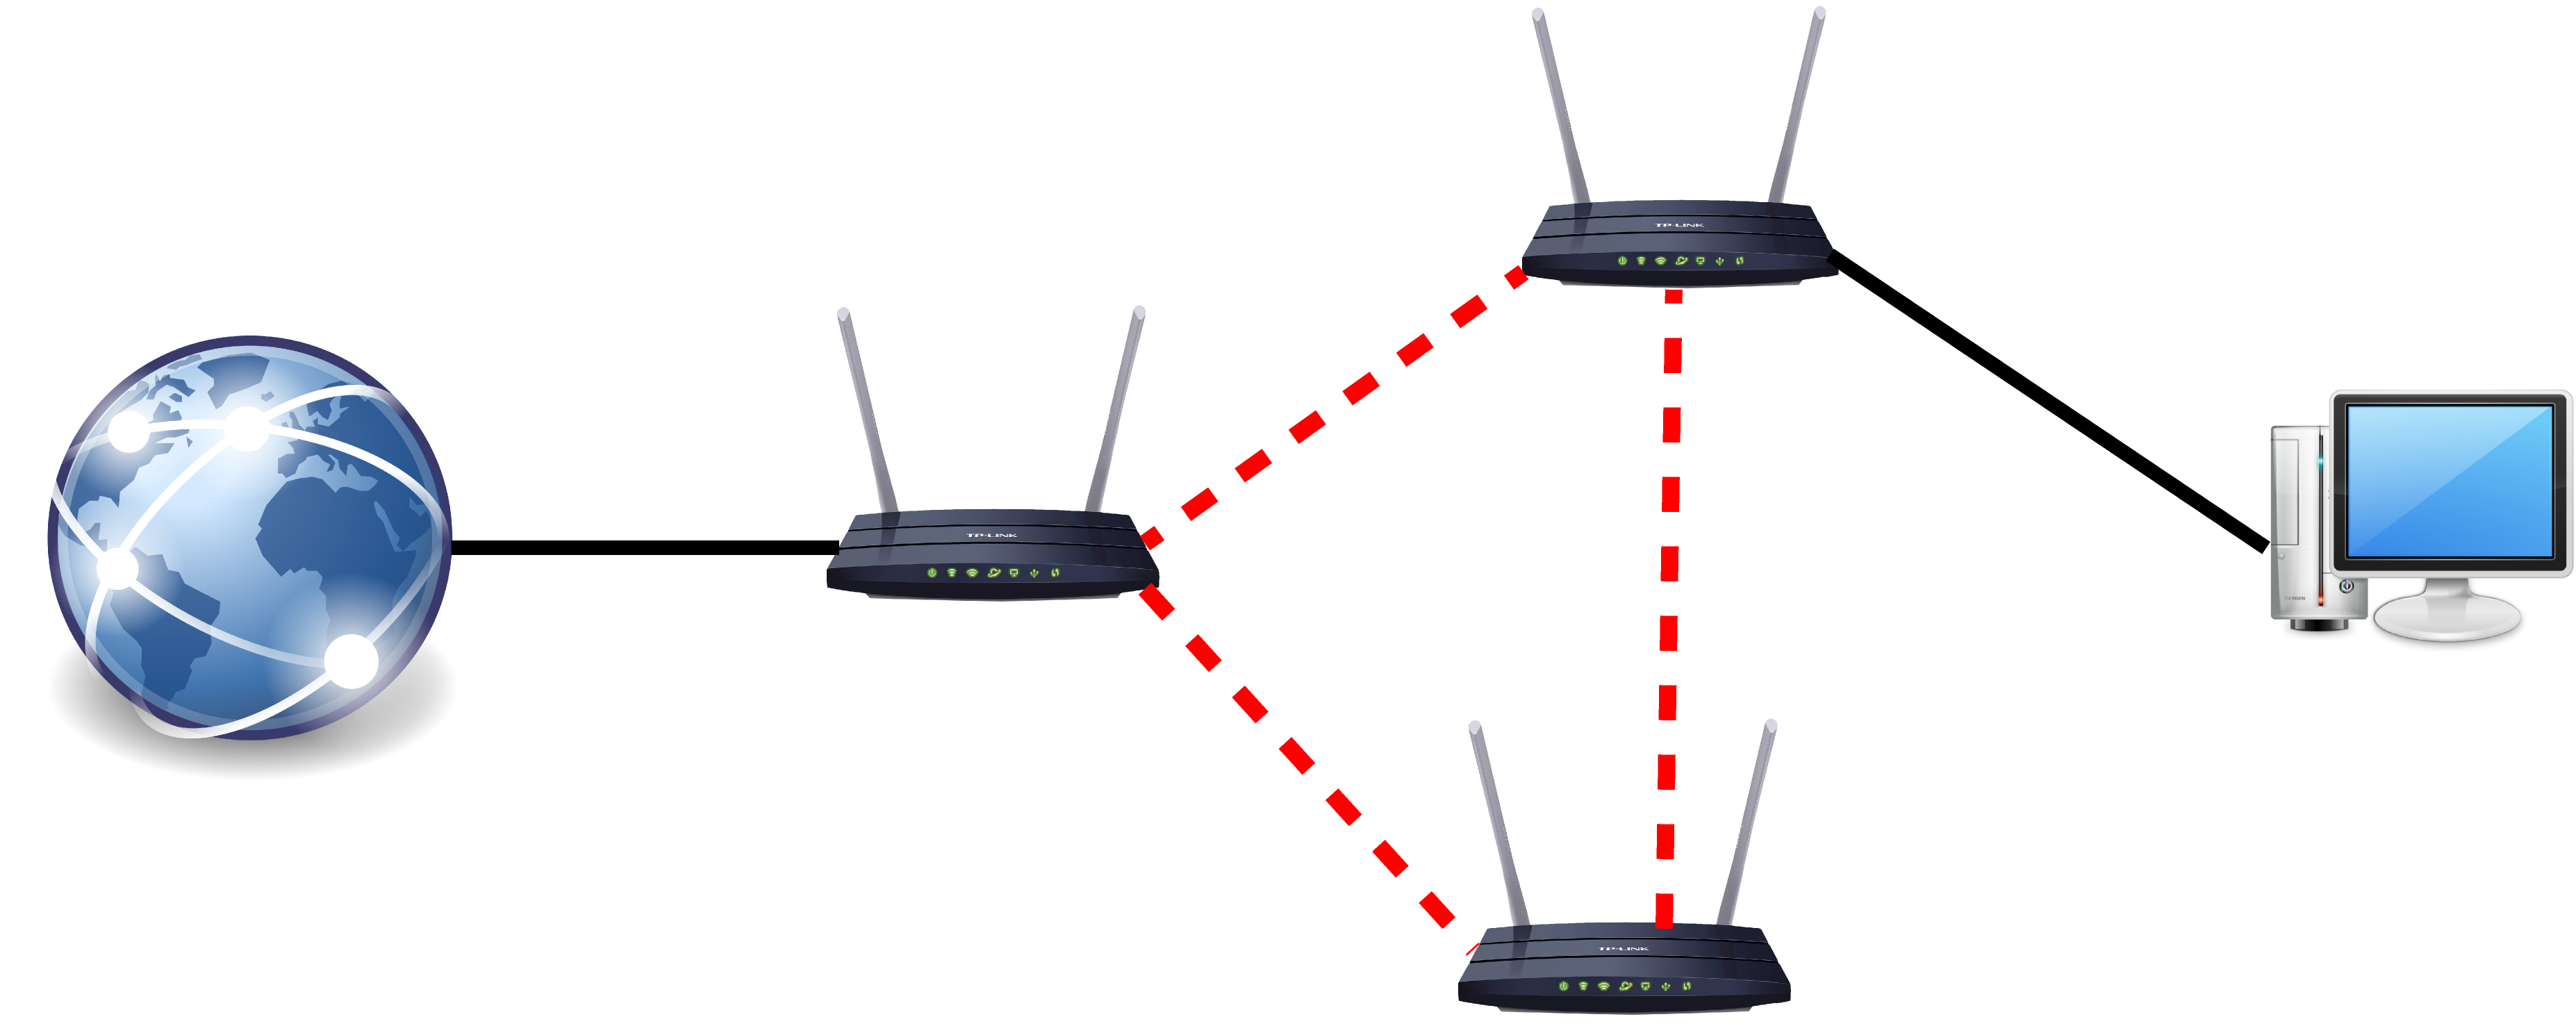
\includegraphics[width=0.7\textwidth]{./figures/RedMeshCasera1.png}		
	\caption{\textit{Topología de primer red mesh realizada.}}
	\label{RedMeshCasera1}
\end{figure}






 
% Chapter Template

\chapter{Conclusiones} % Main chapter title

\label{Chapter2} % Change X to a consecutive number; for referencing this chapter elsewhere, use \ref{ChapterX}

%----------------------------------------------------------------------------------------
%	SECTION 1
%----------------------------------------------------------------------------------------




 
%% Chapter Template

\chapter{Bibliografía} % Main chapter title

\label{Chapter2} % Change X to a consecutive number; for referencing this chapter elsewhere, use \ref{ChapterX}

%----------------------------------------------------------------------------------------
%	SECTION 1
%----------------------------------------------------------------------------------------

%\bibliography{example}
\printbibliography

 

%----------------------------------------------------------------------------------------
%	THESIS CONTENT - APPENDICES
%----------------------------------------------------------------------------------------

\appendix % Cue to tell LaTeX that the following "chapters" are Appendices

% Include the appendices of the thesis as separate files from the Appendices folder
% Uncomment the lines as you write the Appendices

% Appendix A

\chapter{Preguntas Frecuentes} % Main appendix title

\label{AppendixA} % For referencing this appendix elsewhere, use \ref{AppendixA}

\section{Qué hace a un protocolo de ruteo mejor que otro? }

blablabla... esto no se si va. Lo deje porque me gusto como se veia en el template. Pero probablemente el apendice vuele al carajo.

%{\small\verb!\hypersetup{urlcolor=red}!}, or

%{\small\verb!\hypersetup{citecolor=green}!}, or

%{\small\verb!\hypersetup{allcolor=blue}!}.

%\noindent If you want to completely hide the links, you can use:

%{\small\verb!\hypersetup{allcolors=.}!}, or even better: 

%{\small\verb!\hypersetup{hidelinks}!}.

%\noindent If you want to have obvious links in the PDF but not the printed text, use:

%{\small\verb!\hypersetup{colorlinks=false}!}.

%\include{Appendices/AppendixB}
%\include{Appendices/AppendixC}

%----------------------------------------------------------------------------------------
%	BIBLIOGRAPHY
%----------------------------------------------------------------------------------------

\printbibliography[heading=bibintoc]

%----------------------------------------------------------------------------------------

\end{document}  
